\documentclass{ltjsbook}
\usepackage{docmute} 
\usepackage{../../myStyle} 

\begin{document}
\chapter{Types of Numeric Data}
\label{m02_Numbers}
Last time, we talked about psychology as a science, which deals with quantitative data and advances research. This time, we will discuss what kind of data to collect and how to collect it.
\section{Data and Variables}
In psychology, because it studies things that are not visible to the eye, a model is researched that stimulates the subject believed to have a mind and explains the cause and effect relationship as "if you stimulate (stimulus)$\rightarrow$ due to the mind $\rightarrow$ this is how it reacts (response)" by observing the reaction. Here, stimuli and responses are observable things that exist outside of the research target, the "mind," and are made into data.

Figure \ref{fig::03_01} explains the flow of psychological research. The section on "creating data from stimuli and responses" is called \textit{psychometric methods}. It involves considering what to make into data and how to do so, and there are various variations depending on each field of psychology. For example, in studies in areas such as neurophysiology, the data would be the strength and interval of the electrical response obtained from a measuring instrument. In areas such as cognitive, perceptual, and learning psychology, the data would be measured by a PC, for example, the speed of a subject's key response. In applied areas such as social, educational, and clinical psychology, the data would be the subject's speech, response patterns on questionnaires, etc. Regardless of which area data is acquired from, what is important here is the \textit{reliability} and \textit{validity} of the data\footnote{We will discuss this in detail in Chapter \ref{m06_ctt}.}.

\begin{figure}[ht]
    \centering
    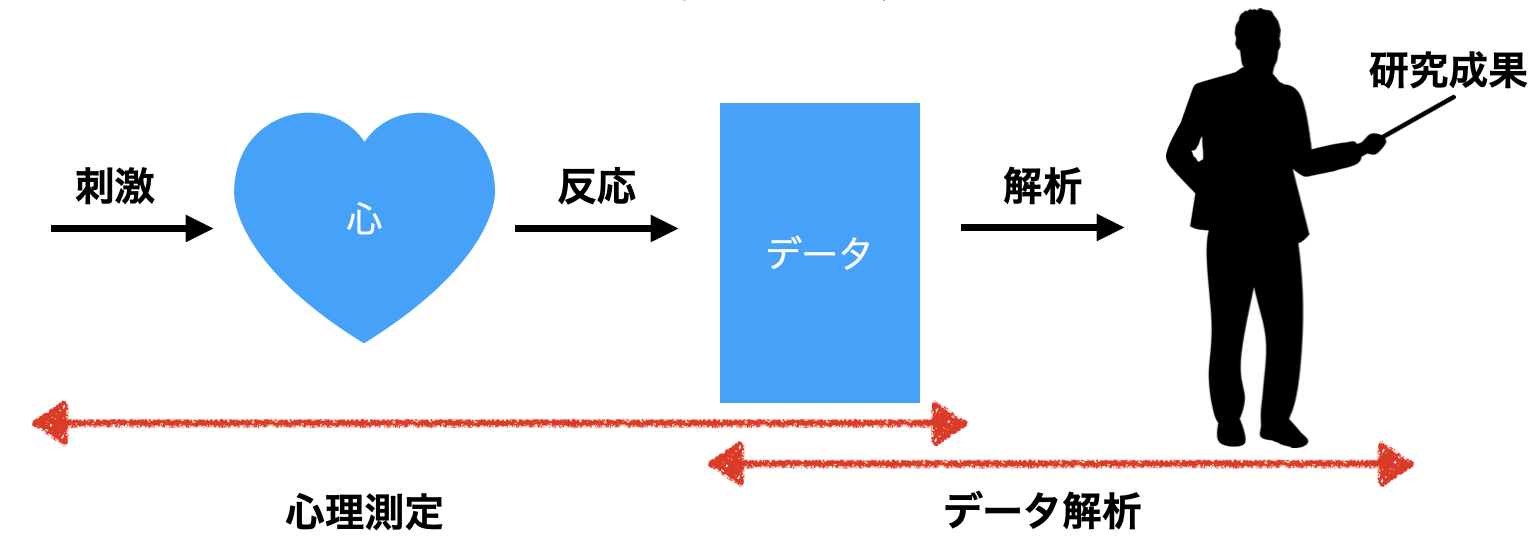
\includegraphics[keepaspectratio,width=0.8\linewidth]{../images/02_Numbers/slide03_01.png}
    \caption{The process of psychological research}
    \label{fig::03_01}
\end{figure}


In this lecture, we will particularly focus on the data analysis section in the latter half. That is, we will discuss how to analyze the data after obtaining it. We will also address this topic in the next session\footnote{$\to$ Section \ref{reproducibility}, Pp.\pageref{reproducibility}}, where the concepts of objectivity and reproducibility are important. It is essential that anyone can arrive at the same results with the same data, and this area also involves making mathematical judgments of correctness or error. Let's learn how to correctly understand and utilize this area.

\begin{figure}[ht]
    \centering
    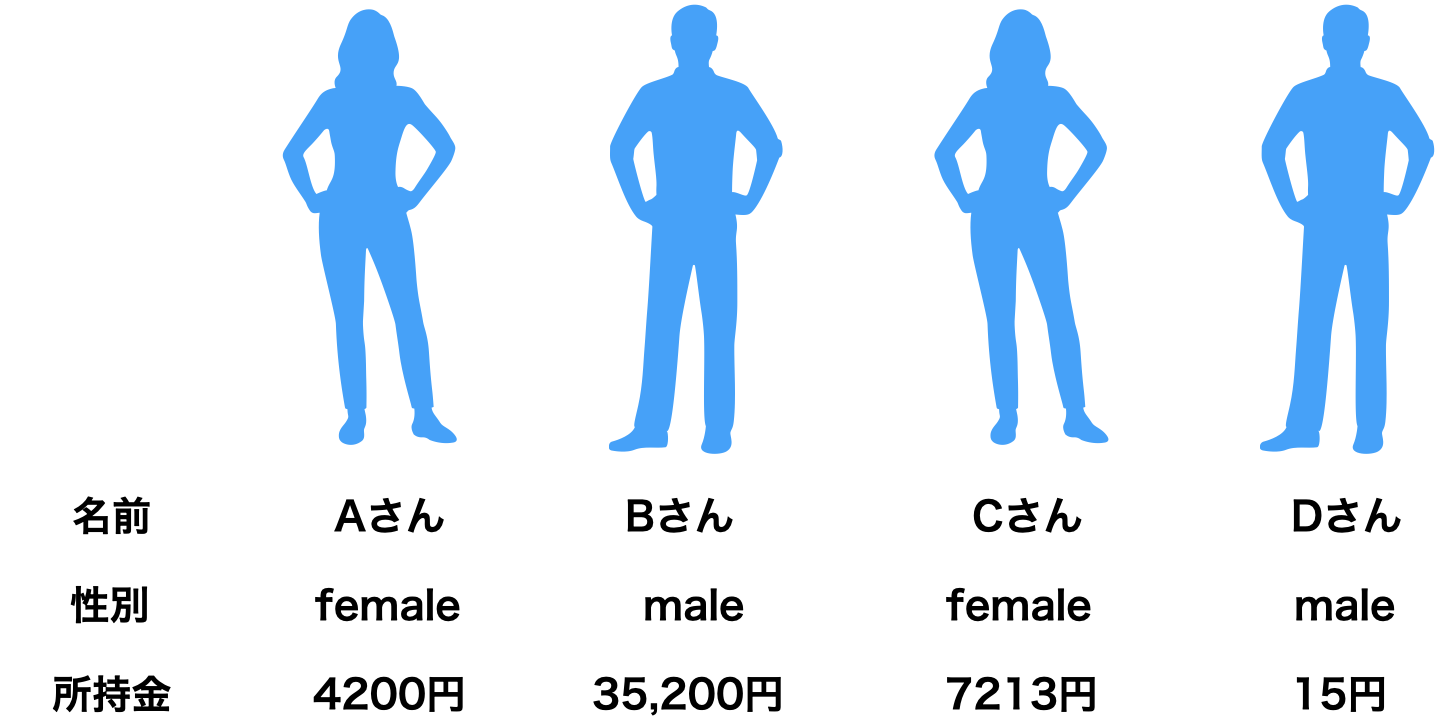
\includegraphics[keepaspectratio,width=0.8\linewidth]{../images/02_Numbers/slide03_02.png}
    \caption{データって何?}
    \label{fig::03_02}
\end{figure}


Now, let's talk about analyzing data. First, what is data? Take a look at Figure \ref{fig::03_02}. There are four research subjects, and we have collected various information about them. But what exactly does "data" represent here? If you think that only the possession of money is data because it is a number, you would be mistaken. In fact, names and genders are also data. All of these can be quantified and treated as data.

I will give you a brief explanation of terminology. Names, gender, amount of money, and so on are numbers that vary from person to person\footnote{In psychology, the unit of data can also be expressed as "individual" or "case" because the research object is not always a person. The abbreviation for "Observation" is sometimes written as "Obs." in English.}. Numbers that vary from person to person are called \textit{variables}. Name, gender, and amount of money are variable names, and they change for each case, such as "Person A," "male," and "15 yen." You may wonder why the name and gender are not numbers. As mentioned earlier, even if it is not a numerical entity, a rule for assigning numbers is determined, and it is replaced with a number. This process is called \textit{scaling}.

\begin{figure}[ht]
	\centering
	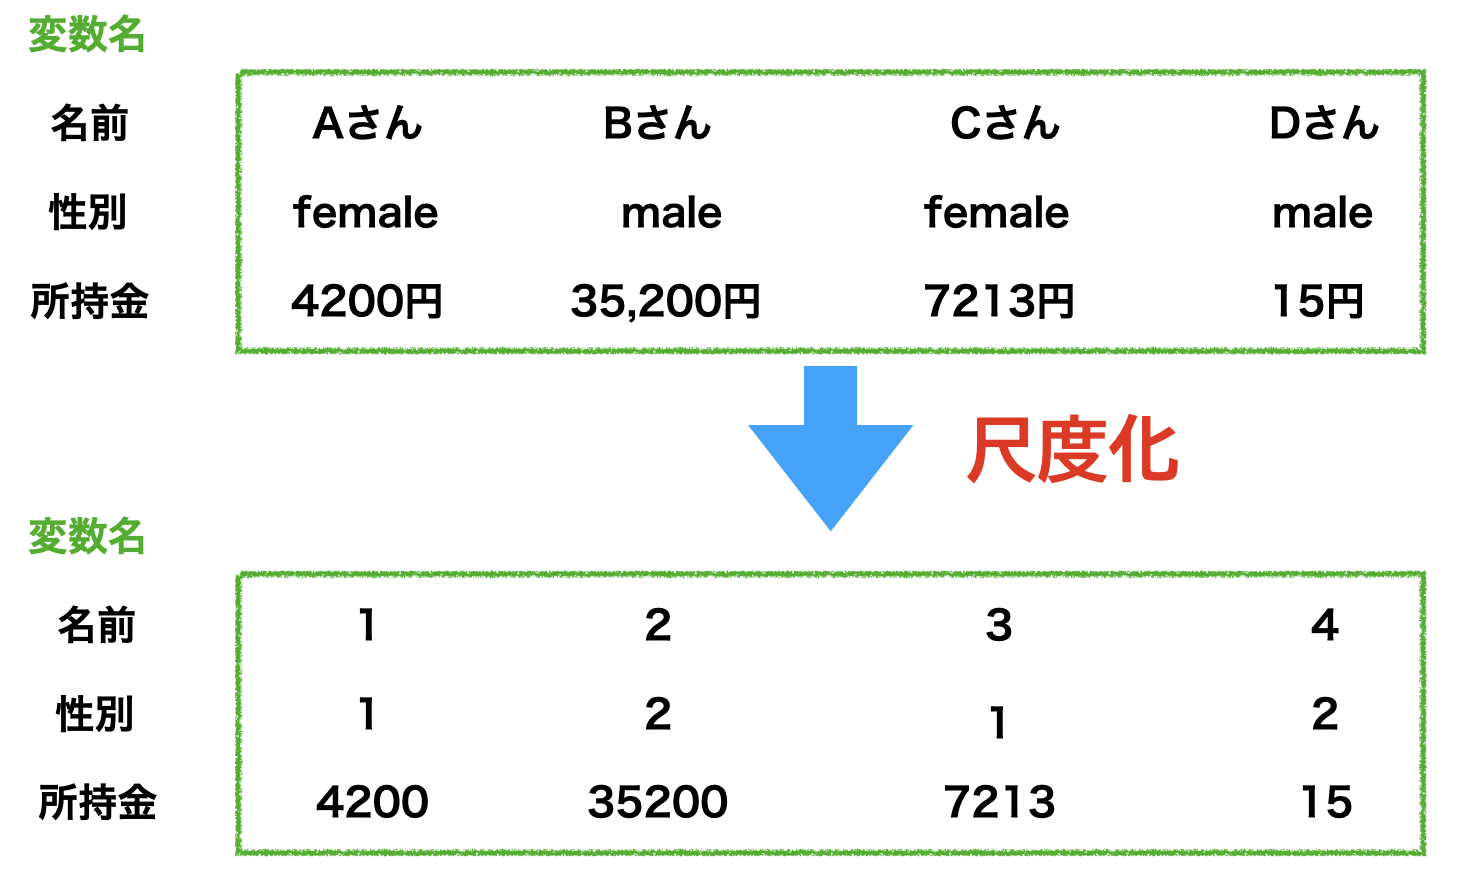
\includegraphics[keepaspectratio,width=0.8\linewidth]{../images/02_Numbers/slide03_03.png}
	\caption{尺度化＝数値に置き換える}
	\label{fig::03_03}
\end{figure}


I have provided an example that has been quantified in Figure \ref{fig::03_03}. The information in the upper row is the original data, while the quantified data is in the lower row. As you can see, the lower row consists entirely of numbers. Let's take a closer look at how things have changed. When performing actual statistical analyses, electronic computers are used. However, when feeding data into an electronic computer, you must understand that it only accepts numbers, as shown in the lower row. Please note that in spreadsheets, such as Excel or Numbers, you can write in Japanese within the cells. However, when working with statistical software, keep in mind that the machine is converting the data into numbers, such as that shown in the lower row. Although within the computer, Japanese characters are reduced to a series of 0/1 binary numbers.

Even just looking at it, you can see that there are two types of numbers. First, take a look at the amount of money. Since this was already a number from the beginning, we will treat it as it is as a number\footnote{The character "yen" for units has been removed. When entering data into a spreadsheet software, it is important to remove anything that is not a number. This is because the software cannot perform calculations with non-numerical values, let alone double-byte characters!}. These types of numbers that have a true numerical value are called \keytermE{numeric variables}. On the other hand, gender is replaced with "1" for "female" and "2" for "male". As for the names, "A" is replaced with "1", "B" with "2", "C" with "3", and "D" with "4". These numbers are used for classifying people and their characteristics and do not represent quantitative differences such as larger or smaller values. They are essentially numbers used to represent qualitative differences, and such variables are called \keytermE{categorical variables}.

As can be seen from this, it is important to note that "even numbers have different types, but they are treated as numbers." Some people might raise their eyebrows at the idea of ​​making everything a number. They might intuitively argue that emotions, feelings, and thoughts cannot be expressed in numbers. However, this is not entirely true because if they can be expressed in words, then appropriate numbers can be assigned to them. Since not all numbers necessarily represent size relationships, it is possible to label them with numbers. On the other hand, there may be feelings that cannot be expressed in words. However, if they cannot be properly expressed in words, they cannot be the subject of scientific research. This is because the statement "the genuine feelings that only I can know" goes against the fundamental stance of science, which thoroughly eliminates privacy. It should be noted that this does not mean that there are no feelings that cannot be expressed in words. I, too, have experienced various changes in my emotions, but those are simply my personal memories and are not the subject of research. Some might argue that by expressing something in numbers, we can only capture a portion of one's emotions. However, avoiding the use of numbers altogether would be a waste. By representing emotions with numbers, we can express what can be expressed, estimate the magnitude of the errors, and touch upon what cannot be expressed, as mentioned in Lecture \ref{m06_ctt} and beyond in this course. It is not constructive to forbid expression altogether.

One research method in psychology is the questionnaire method. It usually consists of multiple items, and respondents are asked to circle one of the following options for each item: "Strongly Agree," "Somewhat Agree," "Neither Agree nor Disagree," "Somewhat Disagree," or "Strongly Disagree." For example, for the question, "Do you think that in this world, effort will eventually be rewarded?" respondents are instructed to "circle the option that best represents your opinion, feeling, attitude, or belief." For instance, one person circles "Strongly Agree," while another circles "Somewhat Disagree." By assigning numerical values to the options, such as 5 points for "Strongly Agree" and 3 points for "Somewhat Disagree," the responses can be quantified and treated as quantitative variables, and the attitudes or beliefs of the respondents towards the fairness of the world can be measured.

By looking at patterns in responses like this, it is possible to quantify invisible mental states. Even though the desired object is an invisible mental state, it can still be measured and given a score. Additionally, all information gathered about desired behaviors and actions can be collected as data, which becomes the subject of analysis.

\section{Classification of Variables}
\label{chap3sec2}
Variables can be classified in various ways according to their context and usage. Earlier we categorized them as quantitative and qualitative variables based on the characteristics of numerical data. There are also differences expressed in terms of "latent variables/observed variables" and "cause variables/effect variables". Let's explain these two differences here.
\subsection{Latent Variables and Observed Variables}
Earlier, I explained a method for replacing individual thoughts and feelings with a numerical scale of their degree of applicability, using numbers that reflect the strength of words in terms of their size and scope (see Figure \ref{fig::03_04}). This process of converting words into numbers with a specific set of rules is known as scaling. There is a solid theoretical foundation behind why "neither agree nor disagree" corresponds to 3, but I will explain that later and move on with the discussion for now.

In the case of psychology, to quantify a mental state (such as depression or level of personality traits), multiple question items are often used to calculate a total score. This is a way of transforming visible data into a substitute for an invisible variable. For instance, grades may be assigned by calculating the total score from the number of correct test answers. This is a form of scaling based on the assumption that the accuracy rate reflects the level of academic ability. Like mental state, academic ability is also one of the assumed invisible mental states.

\begin{figure}[ht]
	\centering
	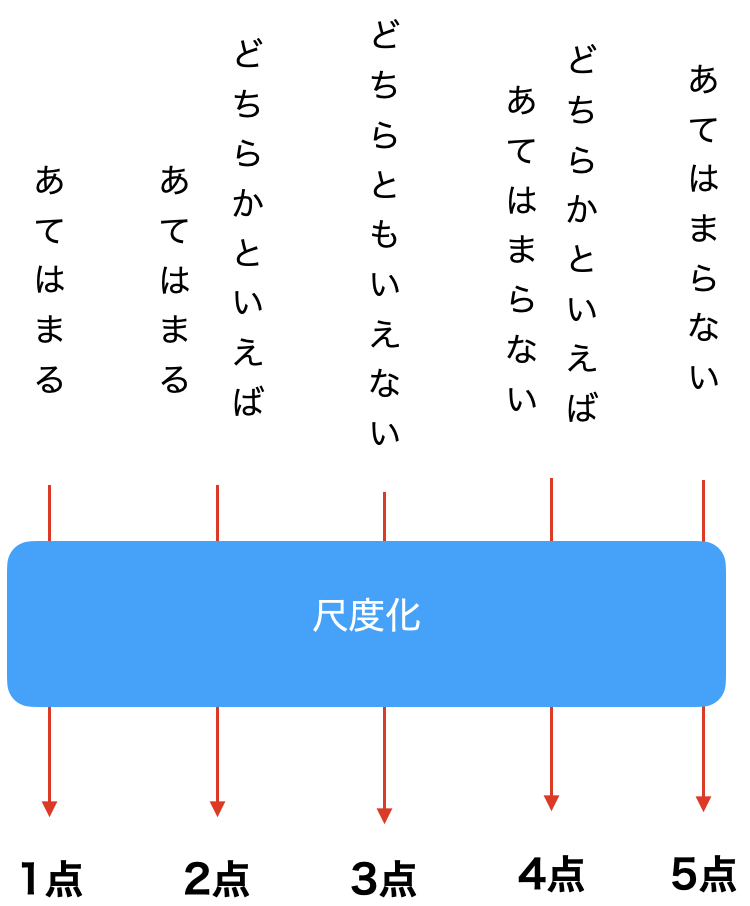
\includegraphics[keepaspectratio,width=0.5\linewidth]{../images/02_Numbers/slide03_04.png}
	\caption{尺度化による数字への置き換え}
	\label{fig::03_04}
\end{figure}


In psychology, we assume a model called "mind" behind human behavior and use visible numerical data called "observed variables" or "outcome variables" to represent it. "Latent variables" are variables representing the state of the model that are calculated from the observed variables. In psychology, we mathematically model measurements and process variables assumed in the models. Latent variables are not represented by specific numbers, but can be computed as abstract models. An explanation of the measurement model is necessary for a more concrete understanding, but it is sufficient to know that we can handle not only observed variables but also other variables.

\subsection{Independent and Dependent Variables}
Sometimes, variables are categorized according to their purpose in research. Consider the following research hypotheses, for example.
\begin{enumerate}
    \item Recording the weight of a young female patient with anorexia who received family therapy for a certain period both before and after treatment. Can we say that family therapy is an effective treatment method?
    \item One group of rats was given free access to food, while the other was subjected to a very low calorie lifestyle. How does the eating style affect lifespan? 
\end{enumerate}

So where do the variables come into play in these cases? The unit of information needed for analysis becomes the variable, so please read carefully and think about it.

In the first example, the timing of measurement becomes one variable because the difference between "before treatment" and "after treatment" is necessary for analysis. Another variable is, of course, weight since we want to know whether or not it has changed. In the second example, it is easy to notice that the length of lifespan (how many days one lives) is a variable, but another variable is the difference between "one group" and "the other group," that is, whether they are free to eat or can only eat low-calorie foods. Without recording this information as data, simply showing the numbers for weight or lifespan length would be meaningless.

The examples presented here all involve verifying the relationships between multiple variables by categorizing them into "causes" and "effects."
\begin{enumerate}
    \item 介入の前と後(原因)$\to$体重(結果)
    \item 食事カロリーの違い(原因)$\to$寿命(結果)
\end{enumerate}

The point is to treat variables as indicators that "change", depending on whether they are pre-intervention or post-intervention data. From the perspective of a research hypothesis, the variables that we want to consider as the cause are specifically referred to as \textit{predictors}, \textit{explanatory variables}, or \textit{independent variables}\footnote{Meaning that they are independent of the outcome.}. The variables that become the result are referred to as \textit{predicted variables}, \textit{explained variables}, or \textit{dependent variables}.

Variables are represented by numbers. For example, 0 represents before intervention, and 1 represents after intervention. If we denote the variable representing before and after intervention as $x$, and body weight as $y$, then this study aims to reveal the functional relationship of $y=f(x)$ with $f$ being the function\footnote{$f$ in $y=f(x)$ stands for function, which can also be translated as "kan-su", meaning both function and operation.}. The fact that psychology is a science, and that being a science involves adopting mathematical positivism and being able to verify models through quantification, is interrelated. Of course, the shape of the function may vary depending on the phenomenon being studied.

Please note that predicting one variable from another using data is only a "hypothesis" of the researcher. It should be noted that since the real truth is unknown, it is possible that the direction of causality may be opposite, even though we consider one variable as the cause and the other as the result. Evaluating whether the hypothesis is correct depends on whether the prediction is accurate. However, since human behavior is complex (or measurement is very difficult), it is not easy to do this successfully.

In addition, causality should come first as the "cause," and the "effect" should come later. In some research, data can be obtained by taking multiple variables simultaneously. From the relationship between multiple variables taken at the same time, we can quantify the strength of the relationship between variables (which will be explained in detail in Chapter \ref{m08_CorrelationCausation}, called the correlation coefficient). However, it is important to note that a correlation relationship does not necessarily mean a causal relationship. A correlation relationship only indicates that there is a relationship between them, and it is not clear which is the cause and which is the result. Causality has a clear temporal relationship. In addition, there may be further causal variables behind the causal variable, or there may be a mediating variable that is common between the causal variable and the result variable. There may be an inverse causal relationship that has not yet been confirmed. Thus, although various things can be expressed from data or numbers, it is ultimately a human problem to interpret them. There are no completely neutral data or models, and we must not forget that they always express some assumptions, premises, or claims.


\section{Classification by Measurement Scales}

You may have seen various names given to variables, but now let's focus on scaled numerical values. It may seem that they are all the same once they turn into numbers, but that's actually not the case. \citet{stevens1946} classified scales into four levels based on the information they convey and the computability that comes with it. Each level has the following names.
\begin{enumerate}
	\item \keyterm{名義尺度水準}{めいぎしゃくどすいじゅん}{nominal scale}
	\item \keyterm{順序尺度水準}{じゅんじょしゃくどすいじゅん}{ordinal scale}
	\item \keyterm{間隔尺度水準}{かんかくしゃくどすいじゅん}{interval scale}
	\item \keyterm{比率尺度水準}{ひりつしゃくどすいじゅん}{ratio scale}
\end{enumerate}


Nominal scale level is at the lowest level, while ratio scale level is at the highest level with a hierarchical structure. Conditions gradually become stronger as you go up the ladder. Conversely, variables that correspond to higher scale levels can be treated as variables at lower levels. I will explain this in more detail later, but let's first explain what each level means.

Nominal scale level
You are at the lowest level of measurement. The numbers at this level are still numeric, but they lack any numerical meaning. We call numbers in this level \textit{nominal scale} when we simply assign numbers as labels to objects. Recall in section \ref{chap3sec2}, Pp.\pageref{chap3sec2}, where we assigned numbers to gender and names. For example, suppose we assign 1 to females and 2 to males. These assigned numbers have no deep meaning. It does not mean that females are twice as many as males or that males are less than or smaller than females in any sense. Your mobile phone number is also at this level of measurement. Your numbers are all different, but they do not have any deep meaning either, except perhaps for ease of memorizing. Similarly, student ID numbers and numbers assigned to names (e.g., A = 1, B = 2, etc.) do not have any numerical characteristics; they are simply a simplification of names. These are called nominal scale numbers.

The numbers at this level cannot be used for calculation, as they do not represent any ordering or sequencing of the data. For example, if we collect data that scale females as 1 and males as 2, the average would be 1.7. However, this number does not have any meaning as there is no object that corresponds to 1.7. In this level of measurement, what is important is that \texttt{each number corresponds to a unique object}, and changing the number will not change its meaning. However, the numbers in this level of measurement are not completely useless, as they can be used for classification since different numbers correspond to different objects. Also, unlike other levels of measurement, nominal measurement can assign numbers to even the most complex objects, providing more information. In addition, as I mentioned earlier, if we cannot express something in words, we cannot study it. Therefore, if we can put it into words, we can assign nominal measurement numbers to it.

Ordinal Scale Level
Nominal scale level has no meaning as a number, as mentioned earlier. If there is an added condition of order relationship, in other words, if there is meaning to the size of the number, then it can be considered as numbers of the ordinal scale level. For example, if someone answers that their favorite dinner menu is curry at 1st and hamburger at 2nd, it can be inferred that curry is preferred, has a higher value, and is prioritized over hamburger. Or, if the numbers represent a ranking of 100m dash, comparing 2 and 7 can reveal that the person who placed 2nd is faster than the one who placed 7th. Numbers with this level of information are called ordinal scale level. However, the numbers of this scale only indicate the size relationship, and nothing else. Even in the case of race placement, it can indicate the winner, second, and third, but it cannot express differences such as “the first place was far ahead” or “it was a relay race”. As shown in Figure 3.5, the data only uses the numbers 1, 2, and 3, so even though the diagrams show different situations, it doesn't differentiate between 2 in the top diagram and 2 in the bottom diagram, and it is still somewhat inconvenient. Since it only provides information about order, it cannot be used for calculations yet. The sum of the first and second place resulting in the third place, as shown earlier, is impossible, and it is unclear if adding 2nd and 3rd can beat the 1st. Of course, it cannot be multiplied, divided, or used for any arithmetic calculation; the numbers of this level cannot undergo any mathematical operations.

\begin{figure}[ht]
    \centering
    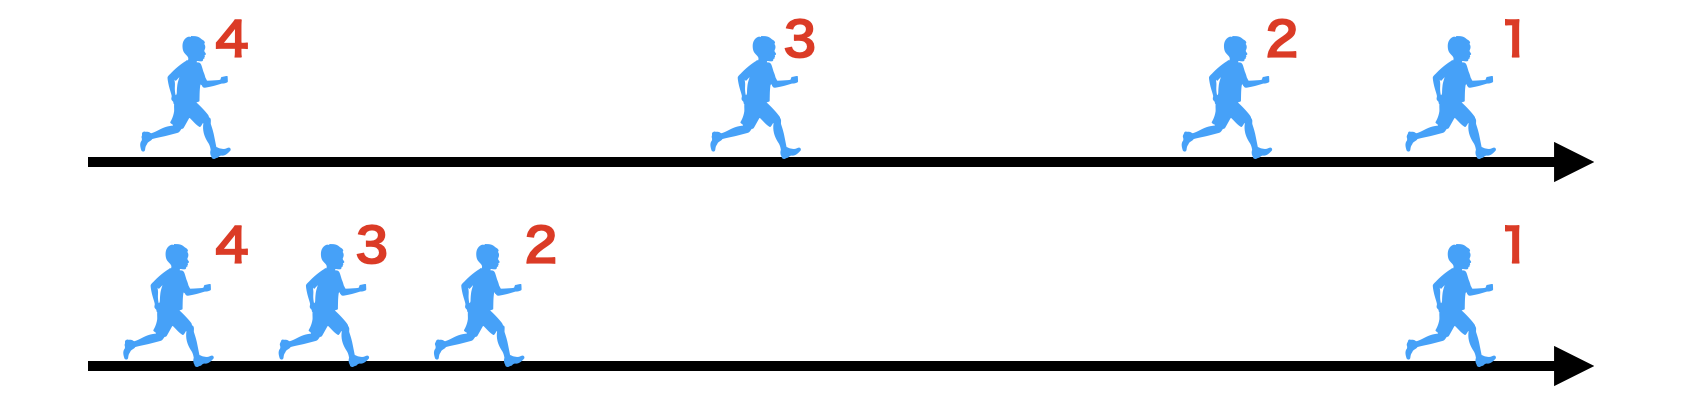
\includegraphics[keepaspectratio,width=0.8\linewidth]{../images/02_Numbers/slide03_05.png}
    \caption{順序では程度がわからない}
    \label{fig::03_05}
\end{figure}


However, these levels of measurement might be the most interesting ones in psychological assessment. If you were to express your own mental state as a number, where would that number lie on the scale? For example, if you thought "curry is 100 times tastier than hamburgers," would that really be an accurate number with a high level of precision? Perhaps assigning five points to curry, four points to hamburgers, and three points to gyoza in terms of preference order would be the most accurate, but it couldn't be said that the difference between curry and hamburgers is the same as that between hamburgers and gyoza. Therefore, the evaluation levels in psychology are at best ordinal measurement levels, and to calculate differences or ratios, higher levels of measurement must be used\footnote{However, in reality, there are often cases where the evaluation values are treated as having the values of interval measurement levels in analysis. This is justified by both the theory of psychological measurement and its historical context. Unfortunately, there are many cases of misuse where they are treated as interval measurement levels without taking them into account.}.

Interval scale level
The \keytermE{interval scale level} adds the condition that the intervals between numbers are equal in addition to the ordinal scale level. While it is acceptable for the ordinal scale level to allow for differences in the interval between 1 and 2 as opposed to 2 and 3, this must be true for interval scale level.
As a representative example, we can consider Celsius (temperature). This expresses temperature using a scale marked with 100 equal divisions between the freezing point of water (0°C) and the boiling point of water (100°C)\footnote{This method is called Celsius because it was invented by Mr. Celsius. By definition, it is like this, so the statement "Water freezes exactly at 0 degrees and boils exactly at 100 degrees, isn't it a miracle?" is a bad joke.}. Since this is a scale that was originally marked at equal intervals, it can be said that the numerical values constitute an interval scale level. At this time, since the difference between 10°C and 20°C is equal to the difference between 20°C and 30°C, we can say that it has reached a level where subtraction calculations, such as $20-10=30-20$, can be performed.

However, it's not accurate to say that 10℃ has twice the amount of heat energy as 20℃. This is because the number 0℃ doesn't hold any value in this comparison. In other words, 0℃ doesn't mean that there's no temperature, but rather it's a particular temperature that exists. The starting point is arbitrary and can be chosen differently, for example.
Let's say we created a new temperature system X, where we set the freezing point at 100 and the boiling point at 200. With this system, 10℃ is equivalent to 110X and 20℃ is equivalent to 120X. Thus, we can see that $20/10 \neq 120/110$, even though these numbers represent the same state. It's strange that our calculations don't match up. In order to perform such division calculations correctly, we will need to add another condition.

Ratio scale level.
The \keytermE{ratio scale} is a level of measurement that, in addition to the interval scale, establishes an absolute zero point. The absolute zero point refers to the point where there is "nothing" at 0. For example, 0 cm represents no length, 0 kg represents no weight, and 0 seconds represents no time elapsed. It is only when a numerical system with a fixed origin of 0 is established that all four arithmetic operations of addition, subtraction, multiplication, and division can be performed. As physical measurement units are almost ratio scale, if measurements are taken with great precision, quite accurate predictions can be calculated. In contrast, subjective evaluation values assigned in psychological data are at most ordinal scale, so there are some areas where they do not work as well as in physics. However, some psychological data can also handle objective numerical values of the ratio scale (such as by using reaction time as an indicator), and subjective evaluation values can be manipulated to become higher than the interval scale with ingenuity.

I believe the type of data that you will analyze in the future will depend on the area of expertise that you pursue. However, it is important to always keep in mind which numbers correspond to which measurement scale. This is because nominal and ordinal measurement scales do not allow for calculations such as addition, subtraction, multiplication, and division, and therefore have limitations in terms of analysis methods. When analyzing data using statistical software, it is also necessary to specify which measurement scale the data belongs to. If the scale is not specified and the machine assumes that all data is capable of being calculated, this can result in absurd analysis. Please refer to Table \ref{tab::03_01} for a summary by Stevens \citep{stevens1946} that outlines the differences between these measurement scales. It is important to note that Stevens' work is not an examination of "what is the appropriate rule for assigning numerical values to the entire measurement target," but rather seeks to determine the rules for converting between various types of measurements, resulting in the four types of measurement scales shown in the table \citep{Yoshino2007}.

\begin{table}[ht]
    \centering
    \caption{Summary of scale levels}
    \begin{tabular}{cccc}
        Scale level & Basic operation & Mathematical group structure & Possible statistics \\\hline
        Nominal   & Homogeneity judgment & Permutation group ($x'=f(x)$ where $f(x)$ is a one-to-one correspondence) & Number of cases, mode, coefficient of coincidence \\\hline
        Ordinal   & Judgment of size relationship & Conformal group ($x'=f(x)$ where $f(x)$ is a monotonically increasing function) & Median, percentile \\\hline
        Interval  & Judgment of equality of intervals or differences & General linear group ($x' = ax + b$) & Mean, standard deviation, rank correlation, product moment correlation \\\hline
        Ratio     & Judgment of equality of ratios & Similarity group ($x'=ax$) & Coefficient of variation \\\hline
    \end{tabular}
    \label{tab::03_01}
\end{table}




From a statistical processing standpoint, both interval scale and ratio scale are considered quantitative data as calculations can be performed on them. On the other hand, nominal scale and ordinal scale are considered qualitative data as calculations cannot be performed on them. Another type of data is count data, which refers to discrete data that only takes positive integers. Additionally, binary data refers to data that only takes on two values, typically 0 and 1. Binary data can have various interpretations such as male and female, true and false, or correct and incorrect, making it a unique type of qualitative data that can also be mathematically calculated like quantitative data despite being at the nominal scale level.

\section{Data Visualization}
\label{dataVisualization}
So far, we've talked about classifying variables and numbers. Keeping these differences in mind, we will now move on to analysis. The first step in analysis is "visualization". Basic rule number one is that "Data must be depicted in charts". You will likely take various data in exercises or as part of research, but don't forget that charting the data is fundamental. This is so important that I will say it twice. In addition, although we will discuss analysis for the next 28 lectures, this emphasis on the importance of "data being depicted in charts" will only apply for this lecture. But, I really want to keep emphasizing the importance of this. As we convey various knowledge and techniques to you during the course of analysis, you may feel that the relative importance of "data being depicted in charts" has decreased, but that is not true. Please create a chart for all data collected, and from various perspectives. Furthermore, even for data that you have not yet collected, try to think about how you can obtain a chart like this, or what data you would need to obtain a chart like this. Visualization makes things easier to understand, and provides hints that you might not have noticed otherwise. You will be able to read various pieces of information from a single chart. That's how important visualization is.

On the other hand, without visualization, it becomes just a series of numbers. I don't think there are many people who like a series of numbers, but perhaps those who do tend to overestimate the value of numbers and don't like staring at numbers they hate? They feel like they've understood the essence of the data just by looking at one number. But that doesn't help to understand the essence of the data. The field of data science is becoming increasingly in demand, but excellent data scientists take plenty of time to visualize and look at the data they have on hand\footnote{One analyst said that he spends about a week visualizing the data and looking at hundreds of graphs to find the right way to analyze the data.}. It's important to be aware of this and not waste time by just doing a predetermined analysis and calculating indicators.

The obtained data essentially needs to be visualized, and analysis begins from there. Reproducibility is also important in this regard. Creating figures by randomly clicking buttons and arriving at a finished product is deficient in reproducibility and cannot be checked. Thus, rules for creating figures are necessary. Spreadsheet software\footnote{Such as Microsoft Excel, Apple Numbers, and Calcs in the freeware LibreOffice.} easily create figures but involve GUI operations. In statistical environments like R or programming languages like Python, figures are drawn through commands (scripts, programs), or CUI\footnote{A command-line user interface. Commands or scripts are individual instruction sentences, with multiple commands comprising a series of instruction sentences known as a script. Collections of scripts are called programs. Programming can also refer to the act of drawing commands or scripts.}. Creating figures is also programming.

In this lecture, we will be using the statistical environment R, which has a package called \texttt{ggplot2}\citep{ggplot2} for creating plots. A package refers to a set of specialized functions that can be added to R for specific analyses or functions. While the concept of a visualization grammar has not yet fully permeated the psychology industry, it is extremely important not only for the aesthetics of the graph but also for logical beauty and reproducibility. Here, we will briefly explain the grammar of graphics. First, let's take a look at some examples of the types of graphs that can be generated.

\begin{figure}[ht]
    \centering
    \includegraphics[keepaspectratio,width=0.8\linewidth]{../images/02_Numbers/ggplot_sample_01.png}
    \caption{ggplot2による出力例1}
    \label{fig::03_06}
\end{figure}


\begin{figure}[ht]
	\centering
	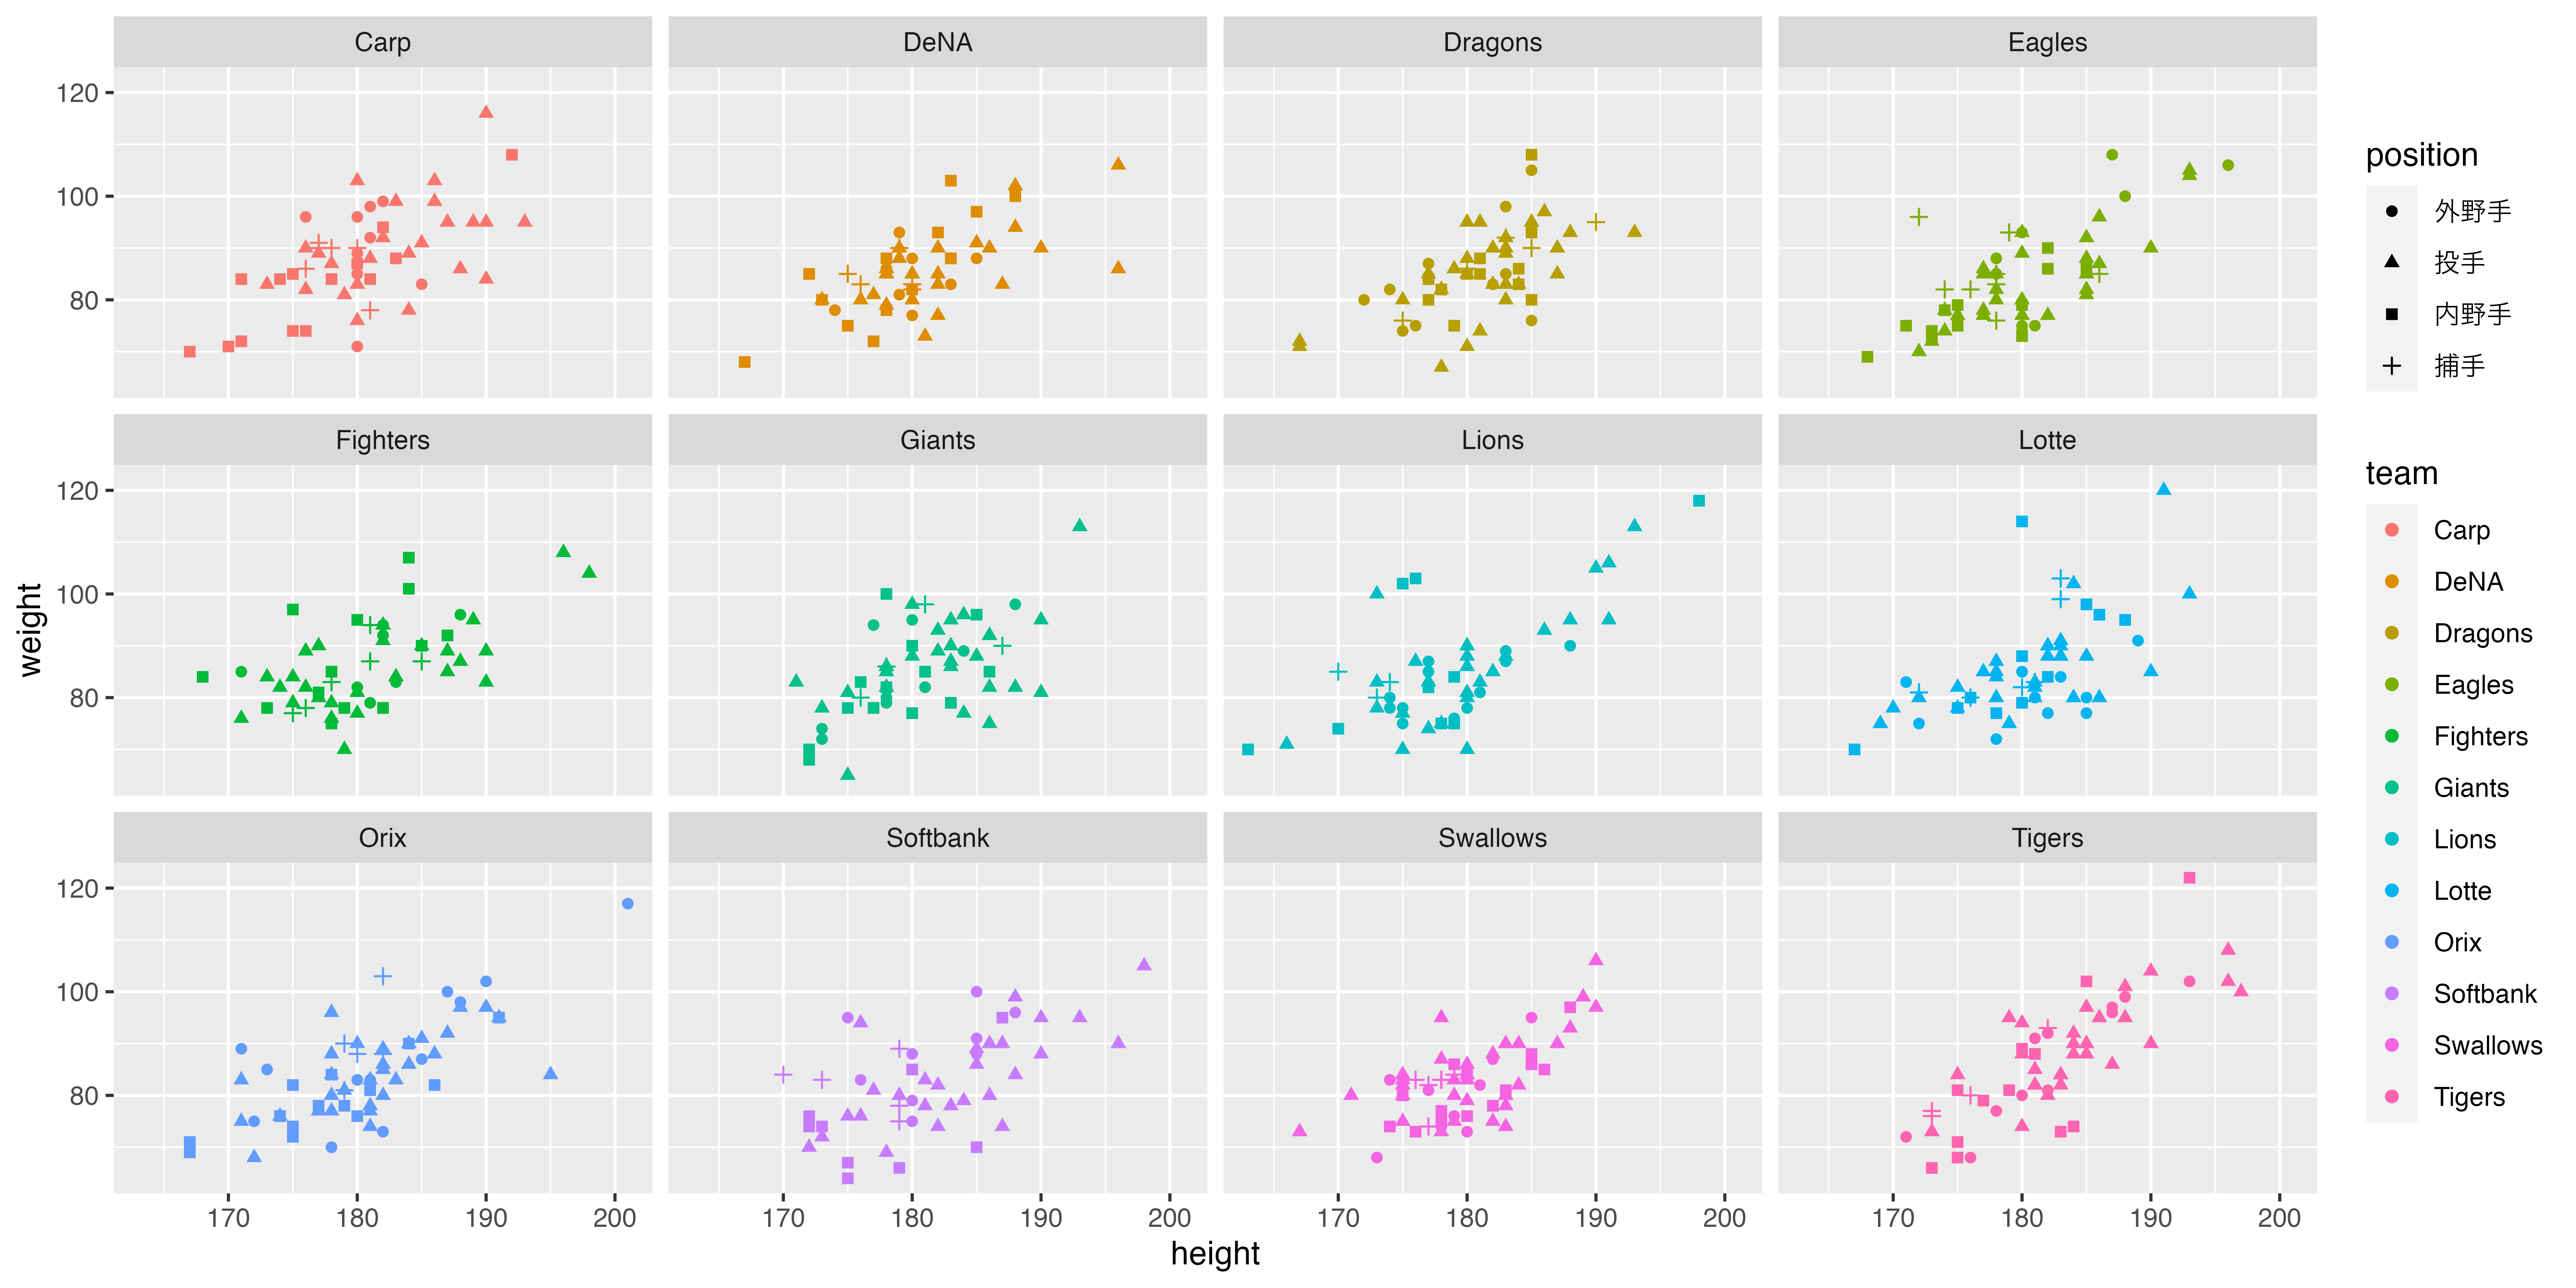
\includegraphics[keepaspectratio,width=0.8\linewidth]{../images/02_Numbers/ggplot_sample_02.png}
	\caption{ggplot2による出力例2}
	\label{fig::03_07}
\end{figure}

\begin{figure}[ht]
    \centering
    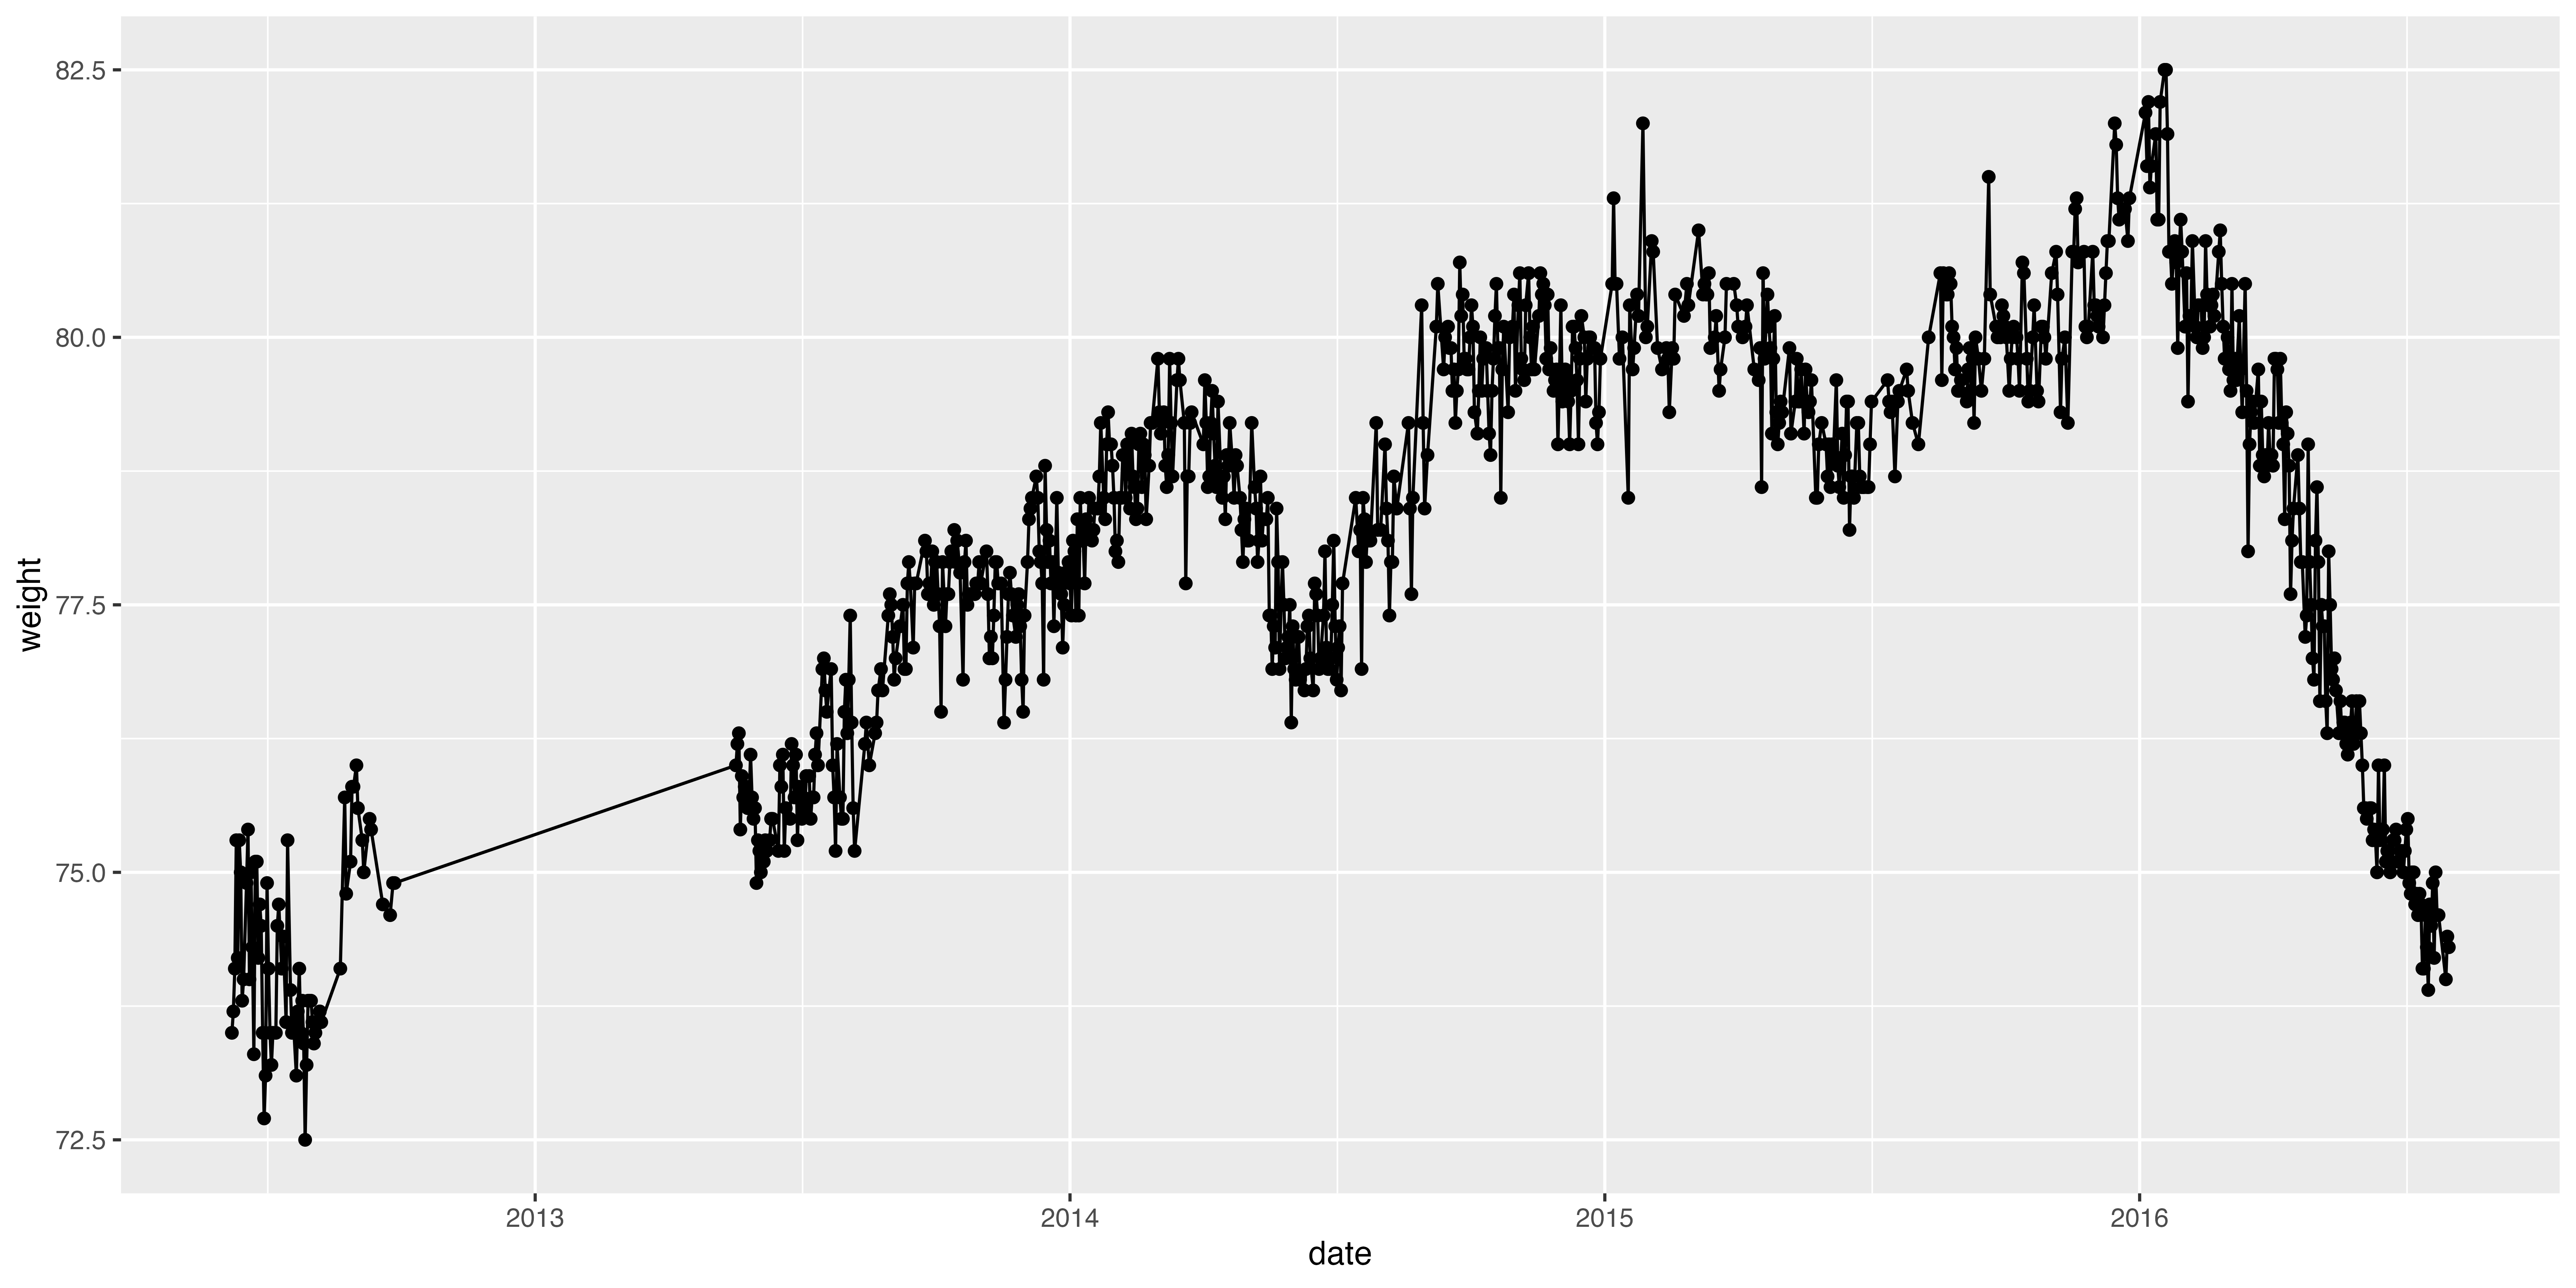
\includegraphics[keepaspectratio,width=0.8\linewidth]{../images/02_Numbers/ggplot_sample_03.png}
    \caption{Output example 3 by ggplot2}
    \label{fig::03_08}
\end{figure}


Multiple plot examples are shown in Figure \ref{fig::03_06}\footnote{The data that this figure is based on summarizes 2020 professional baseball player's height, weight, and annual salary, etc. Here, we show the relationship between height and weight by position and team.}. The scatter plot is located on the top row on the left side. It shows variables on the X and Y axes, and we can visually see how the data is scattered. The points are colored by group. The top right plot shows a box plot, which displays the average and the spread of the data for each of the four groups. The plot in the middle row on the left is the same information as the box plot but presented differently. The data spread is symmetrically displayed as a histogram, and data points are also plotted on top to make it easier to understand. The top middle plot displays a bar plot or a column graph, which represents the average of the four groups by height. The plot on the bottom row is a histogram, which shows the number of data points in each class by height.

The figure shown in Figure \ref{fig::03_07} is a scatter plot, but it is displayed separated by groups. Additionally, the patterns used for plotting were changed for each different label.

The figure shown in Figure \ref{fig::03_08} is a line graph. It displays the record of my weight change, where the horizontal axis represents dates and the vertical axis represents weight. When there is a continuous meaning on the horizontal axis, changes can be represented by connecting each data point.

The purpose here is to make you understand that there are various ways to represent different types of figures, and we will skip the detailed programming methods which will be covered in the Chapter \ref{m03_introR}\footnote{If you are interested, please refer to \citet{Kieran2018} or \citet{Kinosady2021}. There are also various resources available on the Internet, so try searching for "ggplot2".}. What we want to emphasize is that we can embed various types of information by changing labels or colors in a single figure, and these figures are all created using a stack of commands written in a drawing language. Although it is a special language for computers, the shape is created by the machine from the data just by specifying how to draw it in words. Please understand that anyone can reproduce the same figure just by looking at this script, so reproducibility is ensured.

When performing data analysis, it is necessary to create visuals to display the data. One must think about what types of graphs, colors, and shapes will convey information in the most easily understandable way, and design the visuals accordingly. The design process for visuals begins with considering the information to be displayed and preparing it. Then, information is added step by step - determining what will be represented on the vertical and horizontal axes, and what will be conveyed through color, shape, and size. Generally, the design process follows the following steps.
\begin{enumerate}
	\item X軸Y軸にどのような変数を置くかを考える。
	\item X軸Y軸から出来上がるキャンバスに，点や線，何をプロットするのかを指定する。
	\item その上にモデルを加えて，元のデータとの対応を考えたりする。別のデータを重ねることもある。
\end{enumerate}


Let's consider plots and scales of measurement. If both X and Y axes represent quantitative variables, we can use a scatter plot to display their relationship. If the X-axis is a nominal scale and the Y-axis is a quantitative variable, the scatter plot will take the form of dots arranged over the corresponding levels on the X-axis. Figure 3.9 shows two examples of scatter plots; the left one plots two quantitative variables and the right one plots a qualitative variable against a quantitative variable. Even when using the same scatter plot, the appearance can be different depending on the type of variable used. Especially in the case of the right plot, a bar plot that compares the mean values of each level may be easier to convey information than a scatter plot. However, both are still scatter plots, and the fact that the X-axis is a nominal scale will become important in the later discussion, so keep it in mind somewhere in your head.
\begin{figure}[ht]
    \centering
    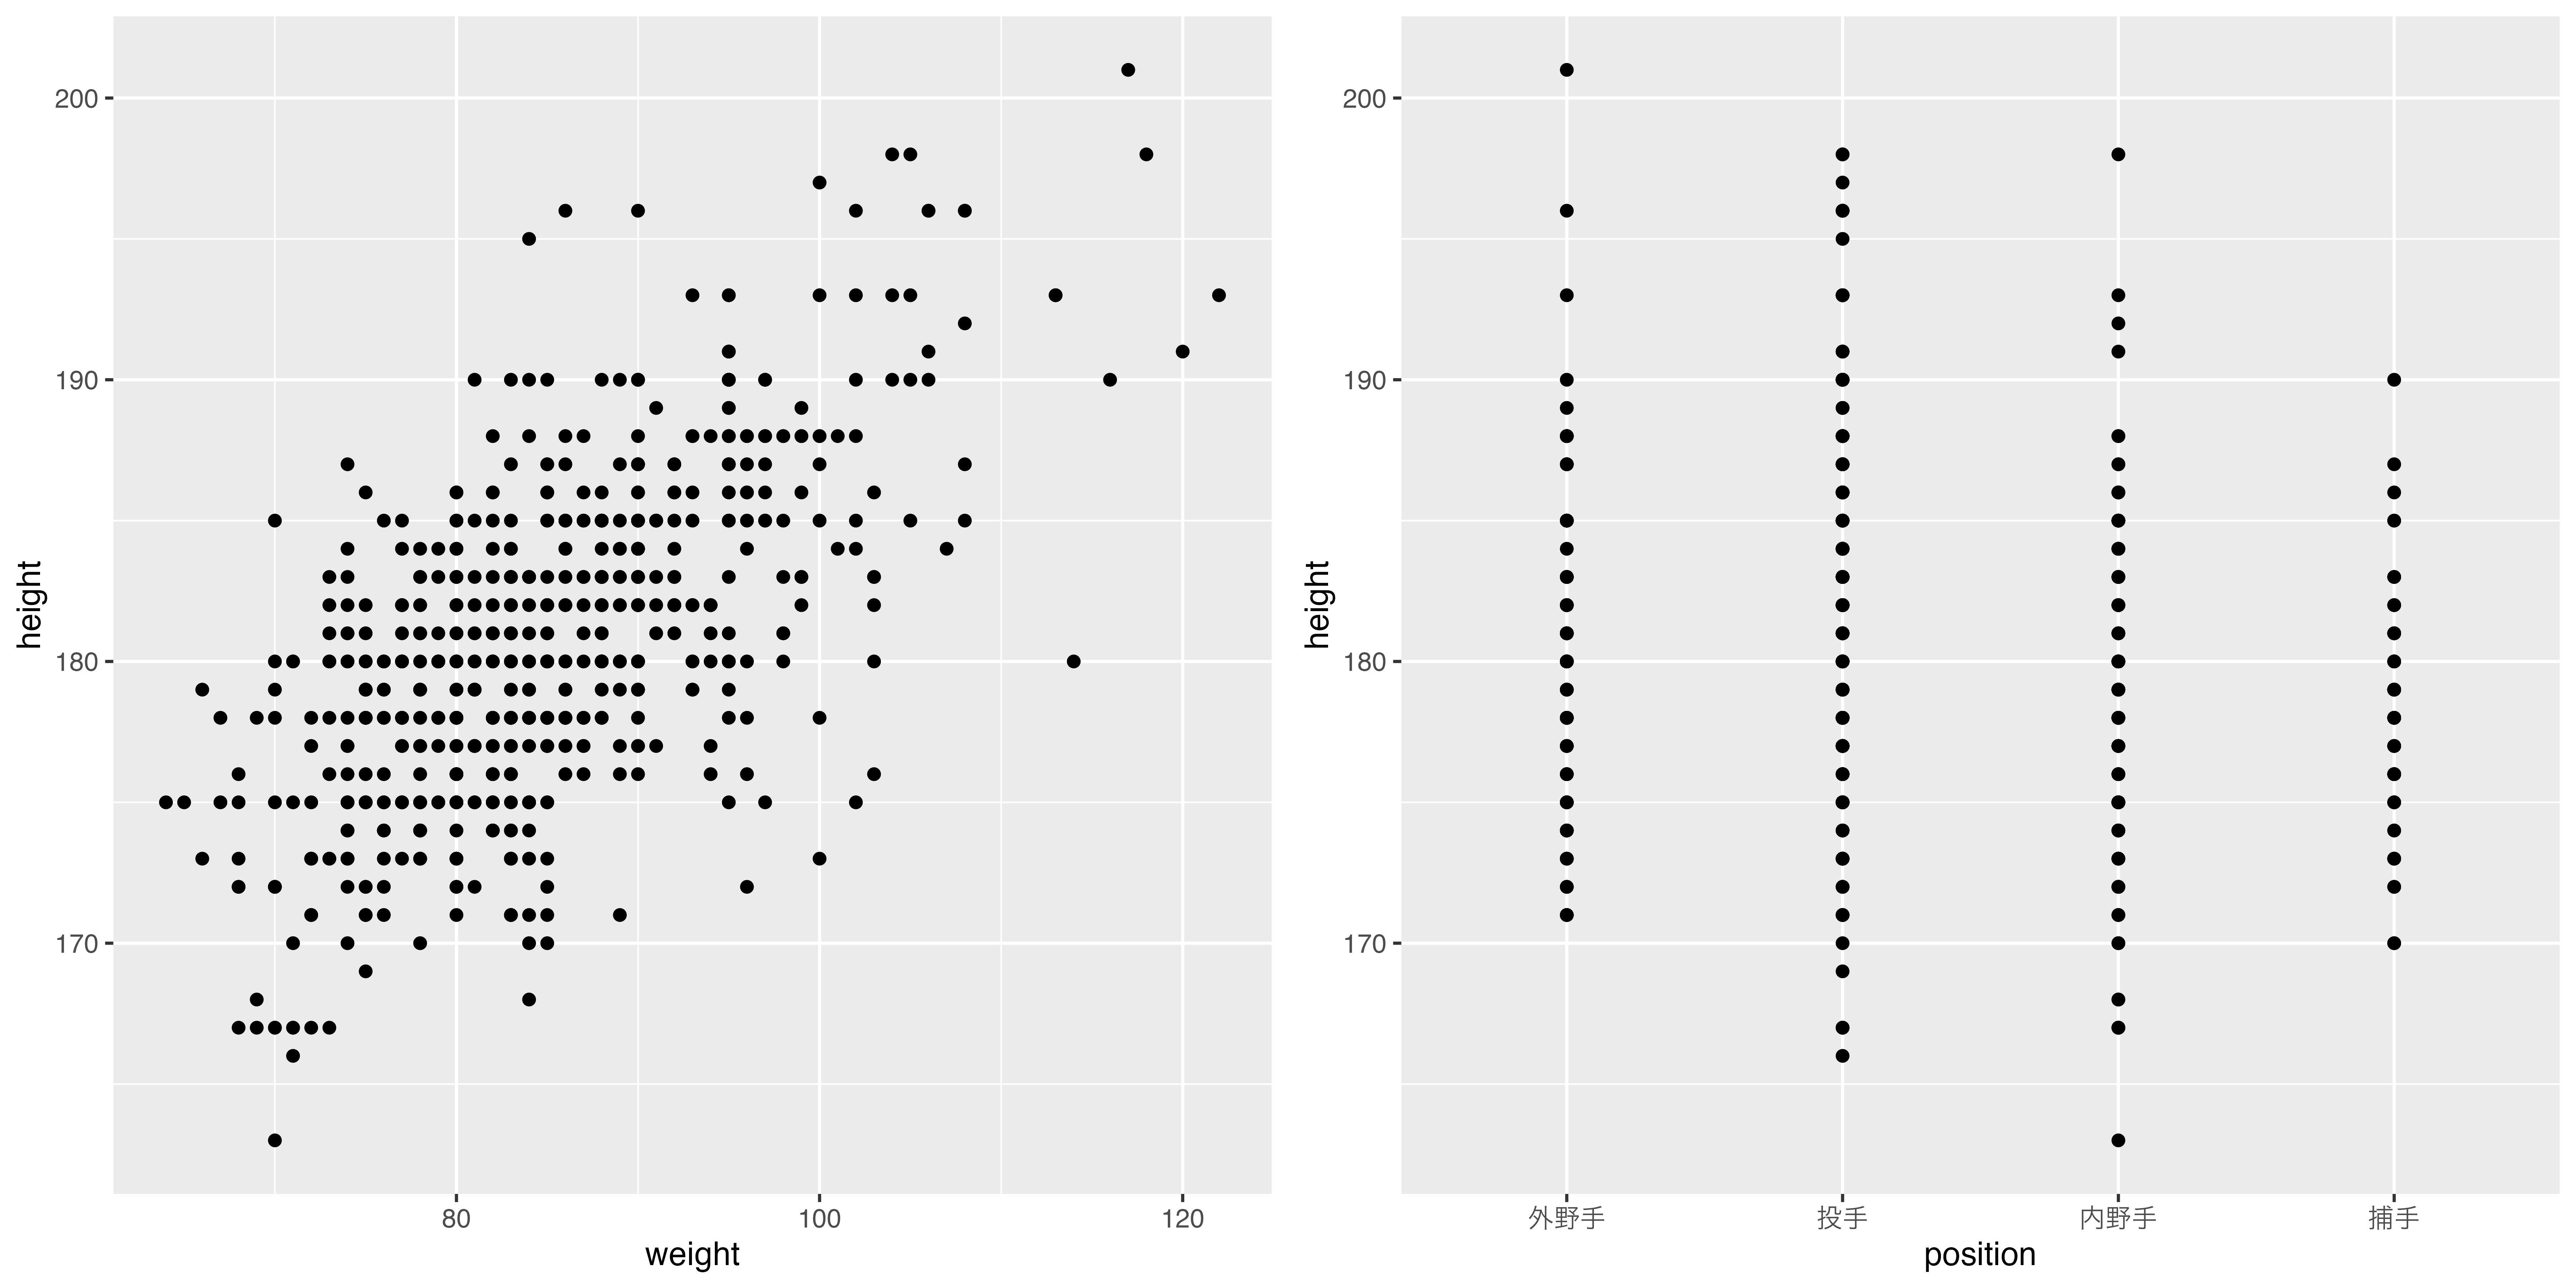
\includegraphics[keepaspectratio,width=0.8\linewidth]{../images/02_Numbers/ggplot_sample_04.png}
    \caption{X-axis and shape of the figure.}
    \label{fig::03_09}
\end{figure}


Some people may think that writing out design procedures just to draw a graph is a tedious task. However, if we consider the reverse of formalizing the syntax of drawing, the benefits become clear. By expressing drawing in words that follow a specific grammar, we ensure objectivity, guarantee reproducibility, and clarify how we intended to represent each set of data. Conversely, hiding our intentions and presenting subjective and irreproducible information is the opposite of a scientific approach. Unfortunately, there are many figures and charts in the world that are created by malicious individuals for the purpose of impression manipulation. While visualizing data helps us understand its characteristics, we may also become misled by visual characteristics and receive different impressions. If intentionally misused, it can mislead discussions. Statistical data, in particular, is an area where it is easy to lie or give false impressions, so caution is especially necessary in this regard.

From the viewpoint of media literacy, there are many good books such as \citet{Takagi196807}.
On the other hand, \citet{Kieran2018} provides a detailed explanation from a perceptual and cognitive perspective on why we misinterpret graphs and charts.
The book by \citet{Kieran2018} is an introductory guide to \texttt{ggplot}, as mentioned earlier, but its first chapter is mostly about psychology.
Please take a look at it as it thoroughly discusses how to present and be seen in what way with examples using the Gestalt principles of visual perception.

\section{Appendix}

For reference, the code for drawing Figures \ref{fig::03_05}, \ref{fig::03_06}, and \ref{fig::03_07} is shown below.
We will cover how to write code in R and their meanings in the 4th lesson (\ref{m04_usingR}).

Note that the data used for the drawings includes baseball player height and weight data (object name in the code is \texttt{sample}) and the author's chronological weight change data (object name in the code is \texttt{weight}) and the code for reading these is not included.

\begin{lstlisting}[language=c++,label={code:03_01},caption={ggplot2による描画コード}]
# 散布図
g1 <- ggplot(sample, aes(x = height, y = weight, 
			colour = team, fill = team)) +
  			geom_point()

# ボックスプロット
g2 <- sample %>%
  select(position, height) %>%
  na.omit() %>%
  ggplot(aes(x = position, y = height, fill = position)) +
  geom_boxplot()

# バイオリンプロット
g3 <- sample %>%
  select(position, height) %>%
  na.omit() %>%
  ggplot(aes(x = position, y = height, fill = position)) +
  geom_violin(alpha = 0.7) +
  geom_jitter(alpha = 0.3)

# バープロット
g4 <- sample %>%
  select(height, position) %>%
  na.omit() %>%
  group_by(position) %>%
  summarise(mean = mean(height), sd = sd(height)) %>%
  ggplot(aes(x = position, y = mean, fill = position)) +
  geom_bar(stat = "identity", alpha = 0.7) +
  ylim(0, 200) +
  geom_errorbar(aes(ymin = mean - sd, ymax = mean + sd), width = .5)
  
# ヒストグラム
g5 <- sample %>% ggplot(aes(x = height)) +
  geom_histogram(binwidth = 1)

g6 <- ggplot(sample, aes(x = height, y = weight, 
            colour = team, fill = team, shape = position)) +
  geom_point() +
  xlab("height") +
  ylab("weight") +
  facet_wrap(~team)

# 折れ線グラフ
g7 <- weight %>% ggplot(aes(x = date, y = weight)) +
  geom_point() +
  geom_line()
\end{lstlisting}




\section{Tasks}
\paragraph{Finding Variables} When devising a research plan like this, what should be recorded as variables?
\begin{enumerate}
    \item From the information about a person's height and weight, we are interested in predicting their gender.
    \item It is said that people sweat a lot while sleeping. We want to investigate whether there is a difference between men and women in the average amount of sweat they produce during one night.
    \item We want to know if there is a difference in happiness between people who are married and those who are not. 
\end{enumerate}


\paragraph{Understanding Measurement Scales} For each of the following data, which measurement scale does it correspond to?
\begin{enumerate}
    \item The numerical value of the last 4 digits of the mobile phone number requested to identify the individual
    \item The personal tax amount for the previous year listed on the tax certificate
    \item As direct questioning of age was awkward, answers were requested for 5 levels: "Teenage", "20s", "30s", "40s", and "50s or older", which were coded as 1, 2, 3, 4, and 5, respectively
    \item Regarding the question, "Strongly agree" was coded as 5, "Strongly disagree" was coded as 1, and the range between the two was equally divided into 2, 3, and 4. "Do not want to answer" was coded as 0.
    \item Celsius temperature, which was developed with the boiling point at 100 and the freezing point at 0, and divided into 100 parts
    \item Temperature is the average kinetic energy of molecules, and as the temperature of a certain amount of substance is lowered, there is a point where it will not go any lower. This is the absolute temperature K that is created based on that point as the origin.
    \item In the TV program "Kaerema 10," the top 10 items from a certain chain restaurant's extensive menu must be guessed. The numerical values represent the popularity ranking for each menu item.
\end{enumerate}


\end{document}
